\chapter{Iteration 1: Design and Implementation}
\label{ch:iter1}

\section{Iteration Objectives}
Prove that a free, keyless data path can discover, store and label Base launches; find whether anything observable at launch predicts the outcome; put whatever survives validation into a live service; and build the interface the proposal showed. Iteration 2 (Chapter~\ref{ch:test} onwards) then proved the signal forward and built the product around it.

\section{Selected Use Cases / Features}
UC1 (watch launches), UC3 (investigate), UC7 (forward record, groundwork), UC9 (trending), and the research pipeline behind FR-1 and FR-2.

\section{Design}
The backend is a set of phases that each read the store and write back through one gate (Figure~\ref{fig:arch}). The phases are separable: ingestion can run without labels, labels without models, and the live scorer uses the same feature code as training (\code{token_features.token_row}) so a live score is computed the way the validated one was. The front end is data-separated: no component invents a value; it renders records from \code{src/data/} or from the API.

\section{Implementation}
\textbf{Phase 1} (11 October) built the package, config, schema and ingestion; the acceptance run backfilled 159 complete 24-hour windows (64,354 transfers, 15,628 swaps, 12,158 wallets) at a measured 44 calls per window and cost nothing. \textbf{Phase 2} (13 October) defined the labels and swept every threshold. \textbf{Phase 3} built the wallet graph (14,528 funding edges, 111,705 co-purchase edges, 134 provable clusters) and validated co-movement lift (4.66, $p = 1.3\times10^{-5}$). \textbf{Phase 4} trained a first model and \textbf{Phase 5 Part A} (18 October) audited it and withdrew it. \textbf{Phase 5 Parts B--D} redesigned the sample (1,066 alive tokens, 841 families, 297,000 keyless calls) and retrained; \textbf{Phase 6} split FAILED and found the buyer-loss target; \textbf{Phase 7} (19 October) shipped the API and the live feed.

\section{Completed Features / Module}
\begin{itemize}
  \item Chain-event discovery and resumable windowed backfill, with budgets and a lookahead-proof write gate.
  \item Outcome labels with stored observations and an offline sensitivity sweep.
  \item A properly sampled dataset with operator families and a data card.
  \item Two validated signals and a shipped artefact with its validation record.
  \item A live scorer and FastAPI service; the Fresh Launches page; the live Trending page; the token page.
\end{itemize}

\section{Technical Implementation Details}
\begin{table}[H]
\centering\small
\begin{tabular}{p{0.34\textwidth}p{0.57\textwidth}}
\toprule
File & What it holds\\
\midrule
\code{blocklens/config.py} & every tunable from the environment: sources, caps, budgets, alert settings\\
\code{blocklens/store/write.py} & the write gate: \code{LookaheadError}, batched upserts, coalescing of nullable columns, product-state writers\\
\code{blocklens/ingest/chain.py} & \code{discover_pools}, \code{backfill_token}: V4 \code{Initialize} and V3 \code{PoolCreated}, 1,000-block windows, V4 swaps by topic filter\\
\code{blocklens/label/rules.py} & named criteria and thresholds; \code{LIQUIDITY_DROP_FRACTION = 0.90}, 90-day window\\
\code{blocklens/label/sample.py} & \code{balanceOf} and \code{extsload} at historical blocks; the V4 token-side method\\
\code{blocklens/sampling/design.py} & windows, strata, families, \code{CUTOFF_BLOCKS = 150} (five minutes)\\
\code{blocklens/model/token_features.py} & the 23 features of \code{t5-2026-10}\\
\code{blocklens/live/scorer.py} & the loop: discover, screen, backfill, score, explain, alert, record, resolve, prune\\
\code{blocklens/live/explain.py} & tree SHAP decomposition, labels, display units\\
\code{blocklens/live/resolver.py} & append-only record, outcomes, scoreboard, paper agent, trade book\\
\code{blocklens/api/app.py} & fourteen endpoints, a session dependency, the SSE generator\\
\code{src/lib/live/*.ts} & typed readers for the API and the public sources; pure arithmetic for the paper book and health\\
\code{src/routes/Launches.tsx} & the feed, push, toasts, notifications, the why-drawer\\
\bottomrule
\end{tabular}
\caption{Key implementation files.}
\end{table}

\section{Algorithms and Technical Decisions}
\begin{description}
  \item[The label.] RUG if the token-side reserve fell by $\geq 90\%$ between consecutive samples within 90 days; FAILED if the price collapsed or trading stopped without a reserve collapse; SURVIVED if it still holds $\geq 25\%$ of peak liquidity and traded on $\geq 8$ of the last 30 days; UNCLEAR below 80\% usable samples; NEVER\_LAUNCHED if it never traded or the pool is degenerate. Each criterion is a named boolean and the verdict one expression, so the sweep can move any threshold.
  \item[Case-control sampling.] A nine-point coarse reserve read (18 calls) selects cases (91\% turn out RUG); a 20\% Bernoulli draw of the rest gives controls; the random cohort, outcome-blind, is the only set at true prevalence and the only evaluation set.
  \item[The model.] \code{HistGradientBoostingClassifier} (depth 3, 300 iterations, learning rate 0.05, L2 = 1.0), Platt-scaled, trained on 593 labelled non-RUG tokens alive at minute 5; a logistic regression is reported beside it. Splits are grouped by family; every confidence interval resamples families.
  \item[Explanations.] Path-dependent TreeSHAP~\cite{lundberg2020} on the shipped ensemble gives one log-odds term per feature; the terms plus the base value equal the model's logit, which a test asserts.
  \item[Budgets.] A token bucket per source (DexScreener 60/min, RPC 4/s, burst 4), a per-run call ceiling, and a persisted monthly ledger.
  \item[Communities.] Louvain with a fixed seed, after greedy modularity failed to finish on 15,000 nodes.
\end{description}

\section{Tools, Frameworks and Technologies}
Python 3.12, FastAPI, uvicorn, SQLAlchemy 2, Alembic, PostgreSQL 16 with TimescaleDB, httpx, scikit-learn, numpy, scipy, networkx, shap, joblib, pytest, pytest-cov; TypeScript 5, React 18, React Router 6, Vite 5, vitest, Playwright; Docker, nginx, GitHub Actions, GHCR, Trivy, Dependabot; TinyTeX for this report.

\section{Demonstration Evidence}
\textbf{The product is deployed and open to anyone:} \url{https://flying-boron-kxx29gy.tmp.now}.
The repository, which always carries the current address, is \url{https://github.com/AbdullahBinNasir16/BlockLens}.

The landing page, the three case studies, Trending Tokens and the wallet screener run entirely in the browser. Fresh Launches, the token page's signals, Paper Agent and Model Health read the BlockLens API, so they report the API as unreachable unless the API is running: during the demonstration it is started with \code{uvicorn blocklens.api.app:app --port 8000}, and the figures below were captured against it. Hosting the API itself is module M11 (Section~\ref{sec:roadmap}).

\begin{figure}[H]\centering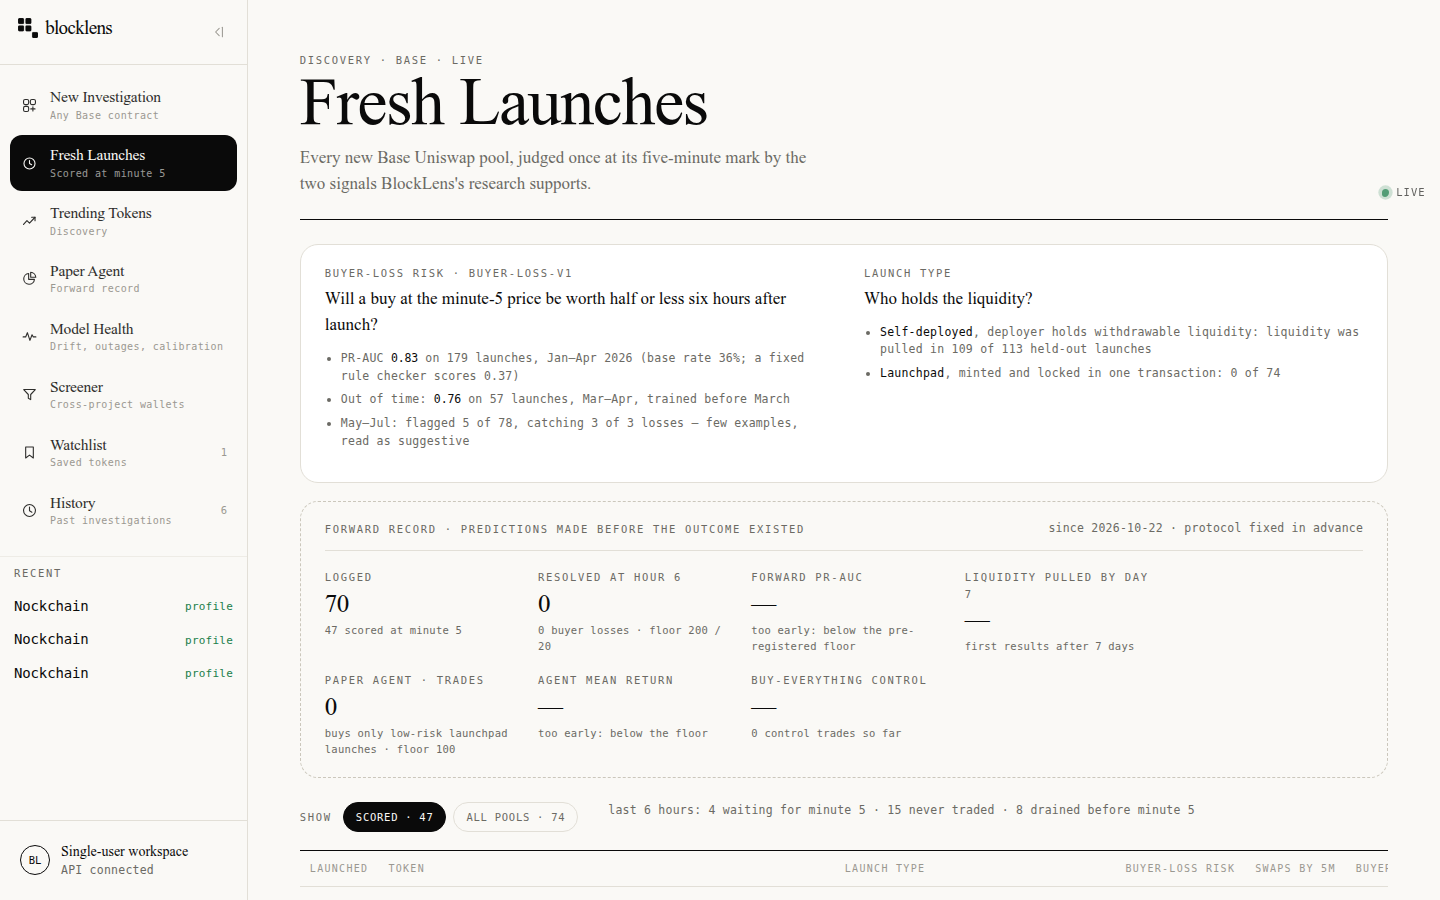
\includegraphics[width=\textwidth]{figures/launches.png}\caption{Fresh Launches: every new Base pool scored at minute 5, with the validation record, the forward record, push status and the why-button.}\end{figure}
\begin{figure}[H]\centering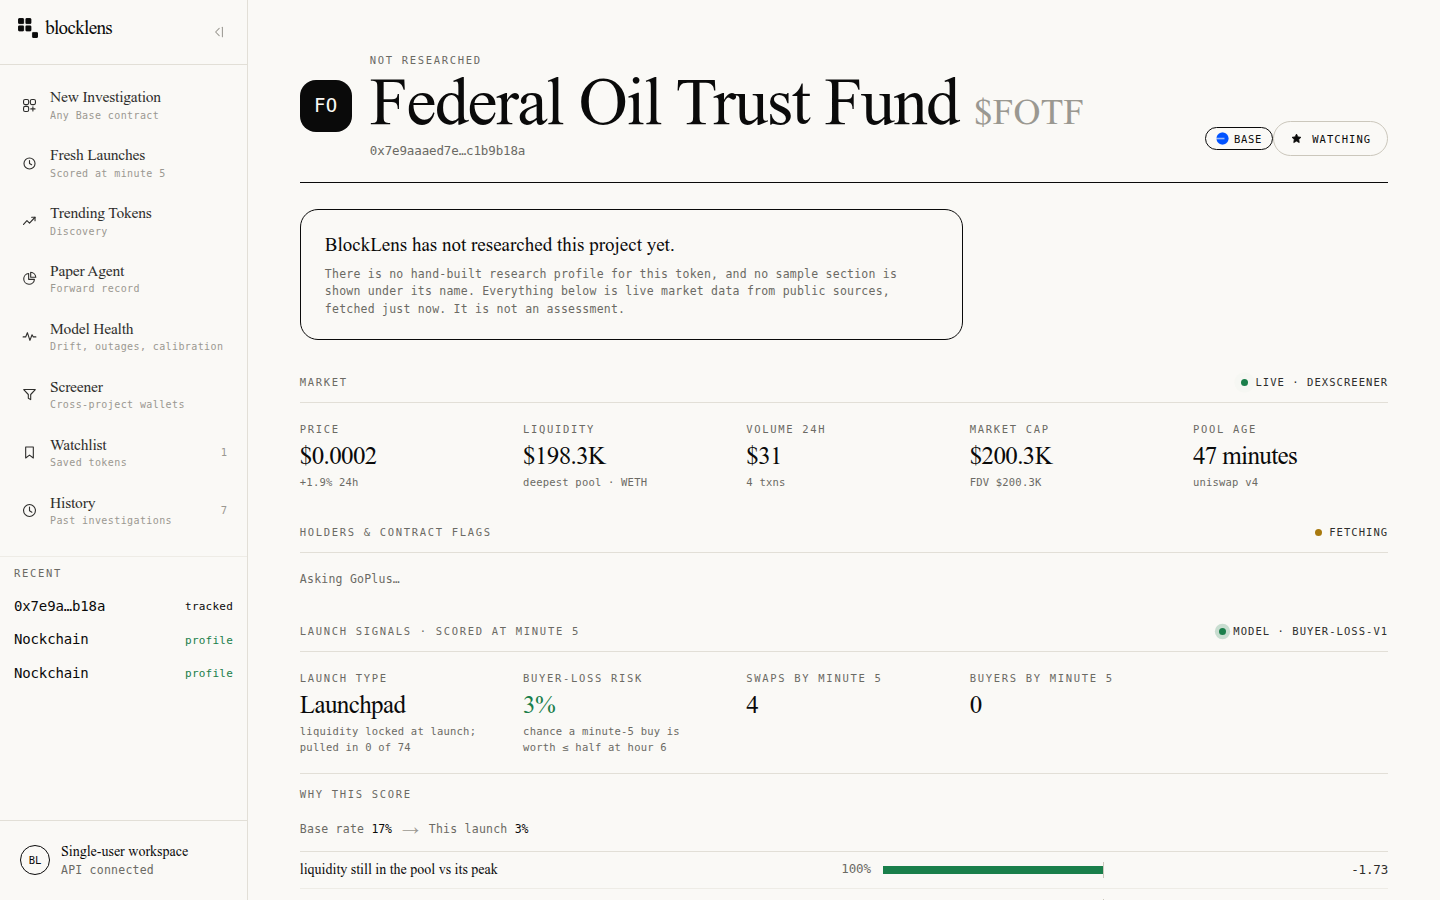
\includegraphics[width=\textwidth]{figures/token.png}\caption{The token page for a tracked launch: live market data, GoPlus flags, the two signals and the score's anatomy.}\end{figure}
\begin{figure}[H]\centering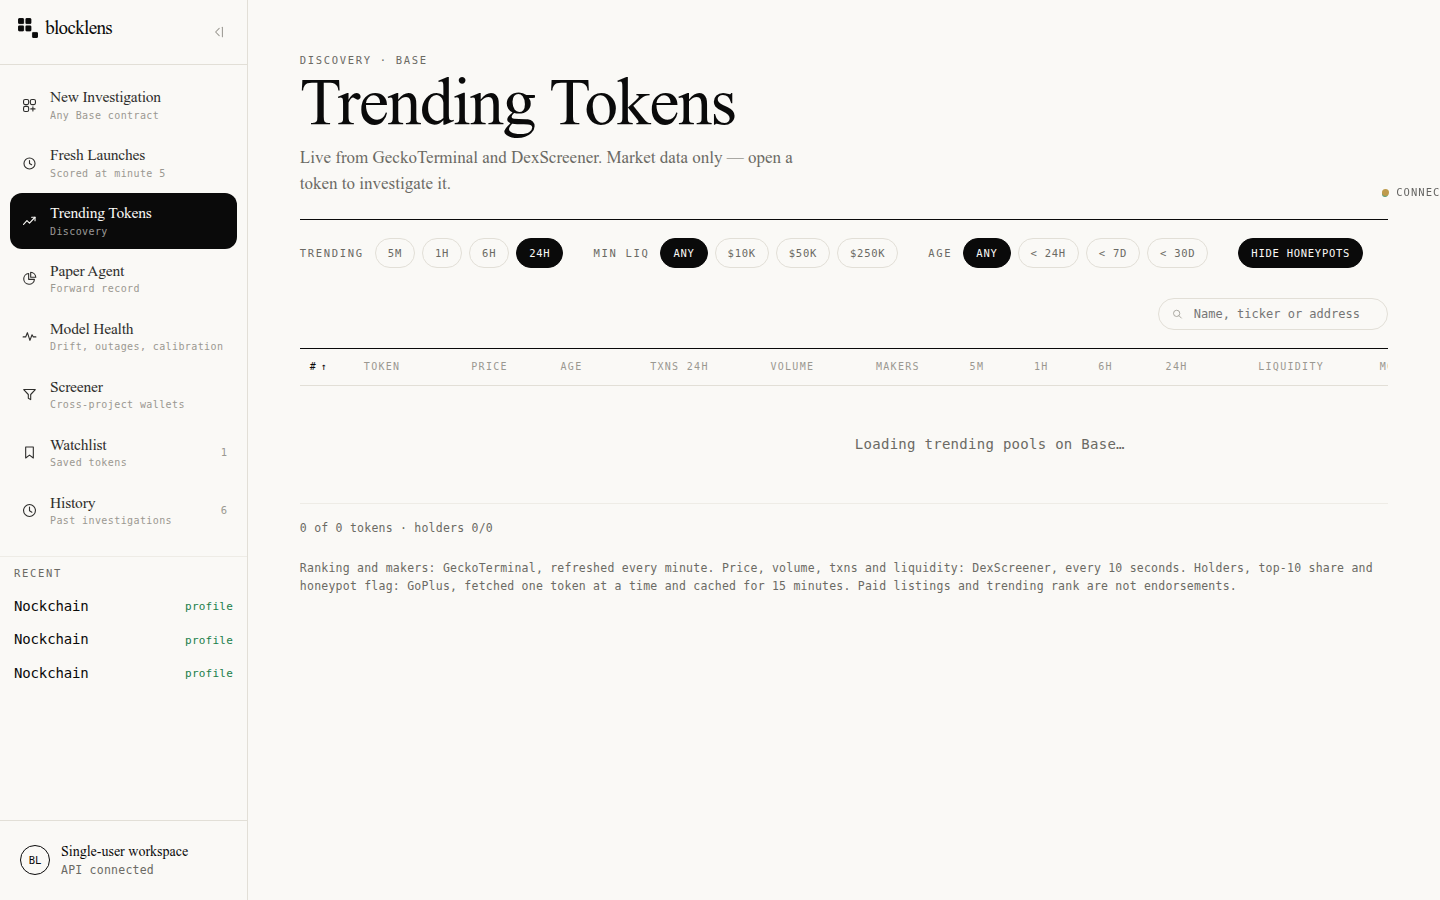
\includegraphics[width=\textwidth]{figures/trending.png}\caption{Trending Tokens over live Base pools.}\end{figure}

\section{Iteration Outcome}
The data path works and costs nothing; the labels are defensible; the first model's result was wrong and was replaced by two signals that hold up out of time; the live feed judges launches within a minute of their five-minute mark. The iteration also produced the project's most important negative result: the wallet graph, which the proposal built on, adds nothing measurable on this population.
